\section{(20점) 클러스터 사용 연습}

\begin{enumerate}[label= (\alph*)]
    \item {
        Fig.~\ref{fig:3-1}와 같이 \texttt{sinfo} 명령어를 실행해보았다.
        이 명령어는 Slurm 시스템의 node와 partition에 대한 정보를 제공한다.
        출력의 각 열은 다음과 같은 의미를 갖는다.

        \begin{itemize}
            \item \textbf{PARTITION}: Partition의 이름.
            \item \textbf{AVAIL}: 해당 partition의 사용 가능 여부.
            \item \textbf{TIMELIMIT}: 하나의 job이 해당 partition을 사용할 수 있는 최대 시간.
            \item \textbf{NODES}: 해당 partition에 할당된 node의 수.
            \item \textbf{STATE}: 해당 partition의 상태(job 수행 여부).
            \item \textbf{NODELIST}: 해당 partition에 할당된 노드의 이름의 목록.
        \end{itemize}


        \begin{figure}
            \centering
            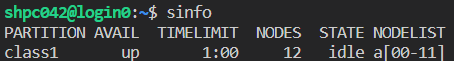
\includegraphics[scale=1]{imgs/Figure06_sinfo_trial.png}
            \caption{\label{fig:3-1}
                \texttt{sinfo} 명령어를 수행한 결과.
            }
        \end{figure}
    }

    \item {
        Fig.~\ref{fig:3-2}와 같이 \texttt{squeue} 명령어를 실행해보았다.
        이 명령어는 Slurm 시스템의 작업 대기열에 있는 작업들에 대한 정보를 제공한다.
        출력의 각 열은 다음과 같은 의미를 갖는다.

        \begin{itemize}
            \item \textbf{JOBID}: 작업의 ID. 각 작업마다 고유한 ID를 갖는다.
            \item \textbf{PARTITION}: 작업이 실행중인 partition.
            \item \textbf{NAME}: 작업의 이름.
            \item \textbf{USER}: 작업을 생성한 사용자의 ID
            \item \textbf{ST}: 작업의 현재 상태.
            \item \textbf{TIME}: 작업이 partition을 사용한 시간.
            \item \textbf{NODES}: 작업에 할당된 노드의 개수.
            \item \textbf{NODELIST}: 작업에 할당된 노드의 이름의 목록.
        \end{itemize}


        \begin{figure}
            \centering
            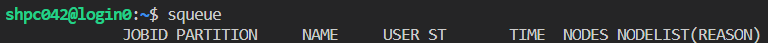
\includegraphics[scale=1]{imgs/Figure07_squeue.png}
            \caption{\label{fig:3-2}
                \texttt{squeue} 명령어를 수행한 결과.
            }
        \end{figure}
    }

    \item {
        Fig.~\ref{fig:3-3}와 같이 \texttt{srun -p class1 -N 2 hostname} 명령어를 실행해보았다.
        이 명령어는 \texttt{class1} partition에서 2개의 노드를 할당받아 
        \texttt{hostname} 명령어를 수행한다. \texttt{hostname} 명령어는 Linux 시스템 사용자의
        이름을 출력하는 명령어이다. 따라서 두 줄의 출력은 각각 할당받은 두 노드의 사용자 이름이다.

        \begin{figure}
            \centering
            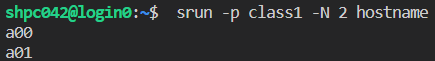
\includegraphics[scale=1]{imgs/Figure08_srun.png}
            \caption{\label{fig:3-3}
                \texttt{srun} 명령어를 수행한 결과.
            }
        \end{figure}
    }
    
    \item {
        Fig.~\ref{fig:3-4}와 같이 \texttt{lscpu} 명령어를 실행해보았다.
        이 명령어는 현재 시스템의 CPU에 대한 정보를 제공한다. 로그인 노드에서 실행했으므로
        로그인 노드의 CPU 정보를 출력한다. 몇 가지 출력만 살펴보면 프로세서는
        AMD EPYC 7502 32-Core Processor이며 L1d, L1i 캐시는 각각 2 MiB, L2 캐시는 32 MiB,
        L3 캐시는 256 MiB이다.
        
        또한 Fig.~\ref{fig:3-5}와 같이 \texttt{srun -p class1 -N 1 lscpu} 명령어를 실행해보았다.
        이 명령어는 \texttt{class1} partition에서 1개의 노드를 할당받아
        \texttt{lscpu} 명령어를 수행한다. 이 경우 컴퓨트 노드에서 실행하게 되므로
        컴퓨트 노드의 CPU 정보를 출력한다. 몇 가지 출력만 살펴보면 프로세서는
        Intel(R) Xeon(R) Silver 4216 CPU @ 2.10GHz이며 L1d, L1i 캐시는 각각 1 MiB,
        L2 캐시는 32 MiB, L3 캐시는 44 MiB 이다.

        두 명령의 출력이 다른 이유는 각자 다른 환경(로그인 노드, 컴퓨트 노드)에서 실행되었기 때문에
        각자의 CPU에 대한 정보를 출력하기 때문이다.

        \begin{figure}
            \centering
            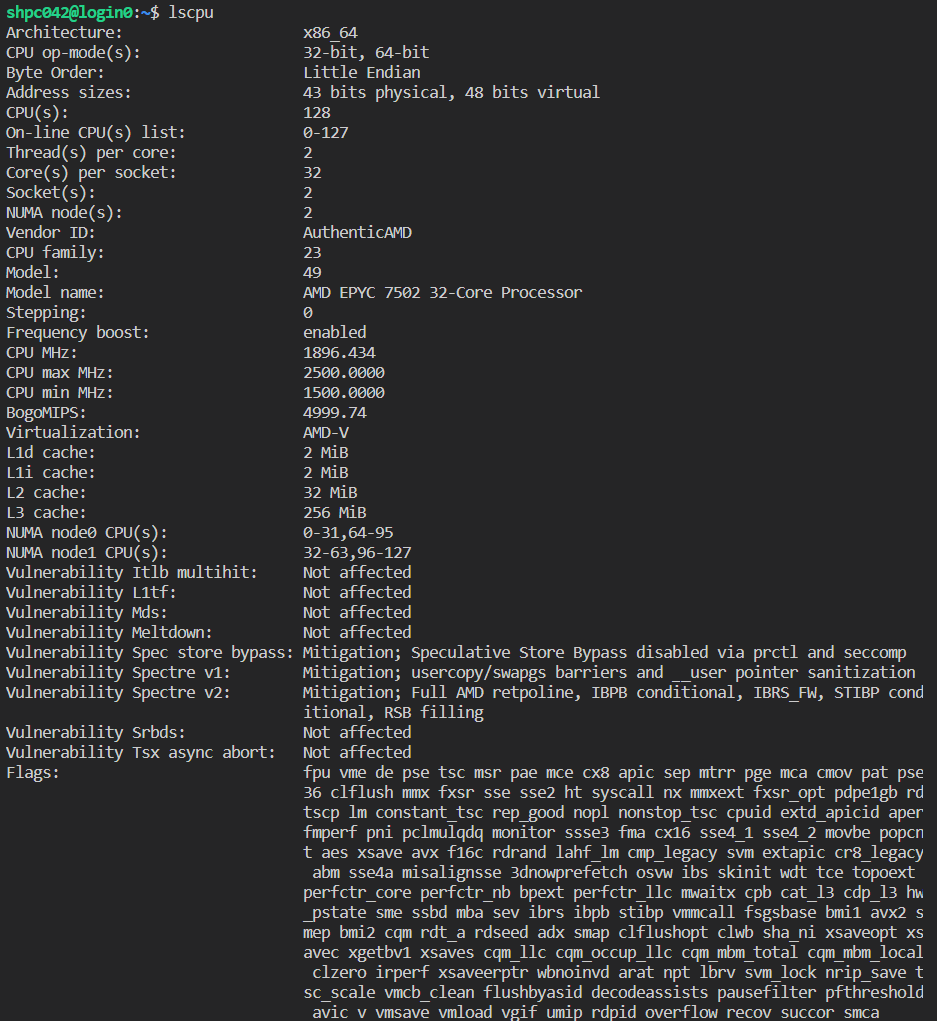
\includegraphics[width=\textwidth]{imgs/Figure09_lscpu.png}
            \caption{\label{fig:3-4}
                \texttt{lscpu} 명령어를 수행한 결과.
            }
        \end{figure}

        \begin{figure}
            \centering
            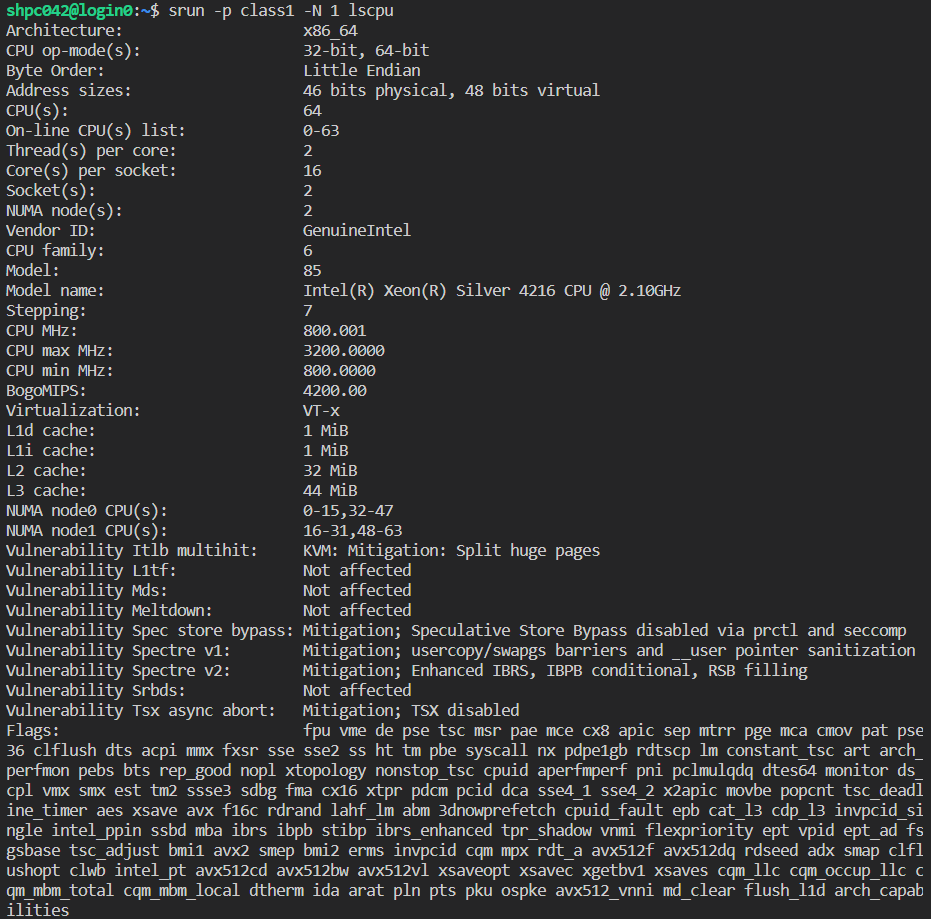
\includegraphics[width=\textwidth]{imgs/Figure10_srun_lscpu.png}
            \caption{\label{fig:3-5}
                \texttt{srun -p class1 -N 1 lscpu} 명령어를 수행한 결과.
            }
        \end{figure}
    }

\end{enumerate}
